

%
% This document has designed to be read through as a PDF first.
% Click on the ``Typeset'' button in the toolbar to generate the PDF
% if it is not already visible.
%

%%% PREAMBLE %%%
% You probably want to skip to \begin{document} if this is your first time.

\documentclass[article,oneside]{memoir}
%% Flip Book \documentclass[20pt]{extreport}
% This command goes at the beginning of every document
% [oneside,article] are two of many options that can be chosen
%   oneside makes each page have the same layout, for printing on only one side 
%     of the paper (change it to twoside to see the difference)
%   article means we're writing a short document only and won't be using special 
%     chapter headings
%   a4paper changes the page dimensions for A4 sized paper 

%%% PACKAGES %%%

\usepackage{graphicx} % Add graphics capabilities
\usepackage{float}
\usepackage{booktabs} % ``Proper'' table layout
\usepackage[fleqn]{amsmath}  % Better maths support
\usepackage[colorlinks=true,linkcolor=red]{hyperref} % Hyperlink capabilities

\usepackage{memhfixc} % This package is required to resolve incompatibilities
                      % with the memoir class & the hyperref package
                      
 \usepackage[T1]{fontenc}
 \usepackage{empheq}
 \usepackage{courier}
 \usepackage{fancyvrb}
 
 \usepackage{caption}  % Required for caption customization
\usepackage[export]{adjustbox}
\usepackage{float}
\usepackage{tabularx}
\newcolumntype{L}{>{\centering\arraybackslash}m{3cm}}


\DeclareCaptionFormat{empty}{} % Define an empty caption format

 
 % Thanks to:
 % https://stackoverflow.com/questions/39856253/numbering-the-subsection-in-latex
 % Answer hbaderts
 
 % Title formating
\usepackage{titlesec}
    \titleformat{\chapter}[display]
        {\normalfont\Large\bfseries}    % Make title \large and bold
        {\huge Chapter~\thechapter}     % Write Chapter X in \huge font
        {20pt}                          % 20pt distance between Chapter X and title
        {}
        [\vspace{1ex}\titlerule]        % Add a line below chapter title
        
          
%\usepackage{pdfsync}
%-----------   \usepackage{/Library/texmf/tex/latex/pdfsync}
% This package is used to tell TeXShop where things are in the PDF file.
% Command-click at any spot in the PDF and it will jump to the corresponding
% location in the source file.

%%% COMMANDS %%%







% Define the title, author and date of the document.
% If the date is undefined, the current date is substituted.
\title {Computing the Singular Value Decomposition (SVD) with Fixed Point CORDIC Operations With  Application to MIMO-OFDM }
\author{Sasan Ardalan Extra Class Amateur Radio, Ph.D.}
\date{}


%%% BODY OF THE DOCUMENT: %%%
\begin{document}
\maketitle
% Generates a title based on the \title, \author, and \date commands in the preamble.
\thispagestyle{empty}
\begin{abstract}
In this paper, the computation of the Singular Value Decomposition (SVD) of complex matrices will be presented. The application of CORDIC operations for fixed point implementations of the SVD of complex matrices will be introduced. SVD plays a major role in Closed Loop MIMO OFDM systems. The impact of fixed point implementation of SVD in a Closed Loop MIMO-OFDM system is examined. The  ratio of maximum to minimum Singular Value (MMSVR) is computed for  both fixed point (CORDIC) and floating point operations (using the LAPACK library). The fixed point implementation  closely tracks the floating point results.  It is shown that for highly ill-conditioned sub carriers the fixed point implementation deviates from the floating point MMSVR. This leads to noise enhancement and degradation of performance. By adding transmit  diversity in Closed Loop MIMO-OFDM the MMSVR can be reduced and performance substantially enhanced for the fixed point implementation. This paper is an important introduction to the algorithms implemented in the GitHub repository for MIMO-OFDM:
https://github.com/silicondsp/mimo-ofdm-release
\end{abstract}
\paragraph{\copyright{Copyright  2006-2025  Silicon DSP$\textsuperscript{\textregistered}$ Corporation}}
Permission is granted to copy, distribute and/or modify this
document under the terms of the GNU Free Documentation License,
Version 1.2 or any later version published by the Free Software
Foundation; with no Invariant Sections, no Front-Cover Texts, and
no Back-Cover Texts. A copy of the license is included in the
section entitled "GNU Free Documentation License".
\begin{figure}[hbtp]
  \centering 
    
\includegraphics [width=0.5in, left]{./Figures/sd-logo-tm_sm.png}
    \captionsetup{labelformat=empty} % Apply the empty format for this figure
  \caption{}
  \label{fig:sdsp}
\end{figure}

\newpage
\paragraph{Sasan Ardalan} received his Diploma from Alborz, Tehran, Iran. He received his Ph.D. from North Carolina State University in Electrical Engineering  in 1983. He was an Associate Professor at NC State in 1991. He was an Adjunct Professor at Duke University.  He has published many articles in  refereed journals in electronics. He has 12 issued US patents.

\newpage
\tableofcontents
 \setcounter{tocdepth}{7}
\listoffigures

\newpage
\chapter{Introduction}



\paragraph{}
In this paper, the computation of the Singular Value Decomposition (SVD) of complex matrices will be presented. In particular, the use of CORDIC operations for fixed point implementations of the SVD of complex matrices will be introduced. This paper is an important introduction to the algorithms implemented in the GitHub repository for MIMO-OFDM:
\paragraph{}
https://github.com/silicondsp/mimo-ofdm-release
\paragraph{}
The C Code written for the Capsim$\textsuperscript{\textregistered}$ Block Diagram Modeling and Simulation tool were written in 2006 through 2016 which also served the basis for the videos on MIMO OFDM in \cite{capsim-mimo} and the MIMO-OFDM Tutorials developed  in 2007  which were published in 2021 on YouTube \cite{ardalan}.

The table below shows various MIMO OFDM Configurations. The beamforming Closed Loop MIMO-OFDM systems with SVD show improved performance over Open Loop MIMO-OFDM systems. Therefore, the fixed point, CORDIC based computation for the SVD of complex matrices, is the architecture that can drive the adoption of the superior Closed Loop SVD systems in Silicon \cite{nasa-ardalan}.

\begin{table}[H]
\small %
\setlength{\tabcolsep}{1pt}
\resizebox{\columnwidth}{!}{
\begin{tabular}{|l|l|l|l|l|l|l|l|l|l}
%\begin{tabularx}{\linewidth}{|l|l|l|l|l|l|l|l|l|l|X }
\hline
\textbf{Configuration} &
  \textbf{Tx} &
  \textbf{Rx} &
  \textbf{CSI} &
  \textbf{FFTs} &
  \textbf{SVD} &
  \textbf{QR} &
  \textbf{Rate} &
  \textbf{Application} &
   \\ \hline
1x1 SISO & 1 & 1 & No  & 1 & No  & No  & 1x & Lowest Data Rate and  Power&\\ \hline
1x2 MRC  & 1 & 2 & No  & 2 & No  & No  & 1x & Longer Range More Power. &\\ \hline
2x2 Open Loop & 2 & 2 & No  & 2 & 2x2 & No  & 2x & Medium Data Rate &\\ \hline
2x2 Beam Forming &
  2 &
  2 &
  Yes &
  2 &
  2x2 &
  Yes &
  2x &
  Medium Date Rate More Reliable than Open Loop &
   \\ \hline
2x3 Open Loop    & 2 & 3 & No  & 3 & 2x2 & Yes & 2x & Reliable Medium Data Rate &\\ \hline
4x2 Beam Forming &
  4 &
  2 &
  Yes &
  2 &
  2x2 &
  No &
  2x &High Down Link Data Rate, Reliable Up-link, Low Power Video &\\ \hline
3x4 Open Loop    & 3 & 4 & No  & 4 & 3x3 & Yes & 3x & High Data Rate  & \\ \hline
4x4 Beam Forming & 4 & 4 & Yes & 4 & 4x4 & No  & 4x & Very High Data Rate &\\ \hline
1x4 Beam Forming & 1 & 4 & Yes & 4 & 4x4 & No  & 1x & Very Long Range \\ \hline
\end{tabular}
}
\end{table}


In \cite{Fredriksson} the performance  of various MIMO diversity schemes  are compared as  shown in Figure \ref{fig:mimo-diversity}.

\begin{figure}[hbtp]
  \centering 
    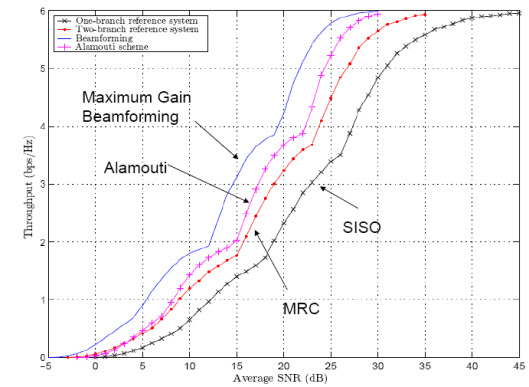
\includegraphics [width=4in]{./Figures/diversity-comparison.jpg}
  \caption{Diversity Schemes MIMO\ \cite{Fredriksson}}
  \label{fig:mimo-diversity}
\end{figure}

The superior performance of the 4x2 Closed Loop SVD MIMO OFDM over the 2x2 OpenLoop MIMO-OFDM \cite{Li} is illustrated in Figure  \ref{fig:mimo-4x2-losed-2x2-openloop}.

\begin{figure}[hbtp]
  \centering 
    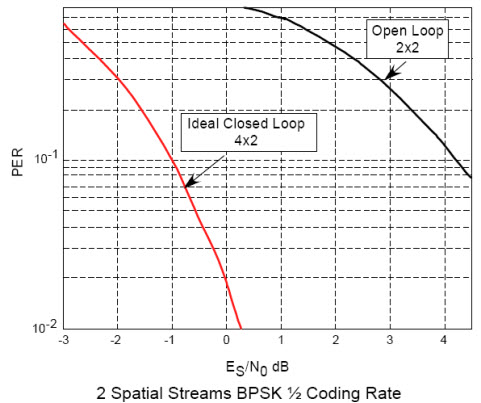
\includegraphics [width=4in]{./Figures/closed_loop_4x2_versus_2x2_open-loop.jpg}
  \caption{Closed Loop SVD 4x2 versus 2x2 Open Loop MIMO OFDM Performance Comparison \cite{Li}}
  \label{fig:mimo-4x2-losed-2x2-openloop}
\end{figure}


\chapter{2	Brief Overview of MIMO OFDM Communication Receiver}
\paragraph{}
A MIMO communication channel is shown in Figure \ref{fig:mimo-channel}. The Figure shows the complex frequency response for a single carrier in a MIMO OFDM system from each transmit antenna to each receive antenna.  The complex elements $h_{jk}$ (j=1, 2, 3) and (k=1, 2) form a complex matrix H. To implement a MIMO OFDM system, the receiver needs to estimate the channel per carrier in order to perform equalization and separate the multiplexed streams (or to generate a single stream in diversity schemes).  To do this, each transmitted packet contains high throughput training symbols. The receiver processes these training symbols and estimates the channel.  In an open loop zero forcing MIMO system, in order to separate and equalize the received channels, the Pseudo-inverse \cite{Weisstein} of the channel is computed for reach carrier’s H channel matrix.

\begin{figure}[hbtp]
  \centering 
    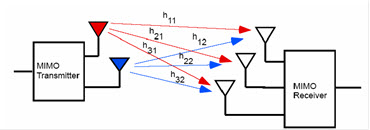
\includegraphics [width=4in]{./Figures/mimo-channel.jpg}
  \caption{2x3 MIMO Per Carrier Channel Model}
  \label{fig:mimo-channel}
\end{figure}

For a comprehensive video tutorial on MIMO-OFDM check \cite{ardalan}.

\chapter{Implementing the Pseudo-inverse for Open Loop MIMO with an SVD of the H Matrix}
\section{Introduction}
We will show that a basic 2x2  MIMO open loop equalizer can be derived from a basic 2x2 Singular Value Decomposition (SVD) of the H matrix. That is, an open loop MIMO system can be implemented with SVD. The key benefit is that for beamforming we use SVD and the SVD computation engine can be used for Open Loop systems. 
\section{Derivation of SVD Based Computation of ZF Equalizer}
The MIMO Zero forcing equalizer is computed from the estimated MIMO channel using the Pseudo Inverse.

\begin{equation} 
  W=H^{+}=(H^{\dagger} H)^{-1} H^{\dagger}
\end{equation}
The streams are equalized from the received streams $\textbf{y}$ .
\begin{equation} 
\hat{x}=W\textbf{y}=\textbf{x}+W\textbf{n}
\end{equation}
Compute the SVD of $H$ and substitute for  $H$.
\begin{equation} 
H=U\Sigma V^{\dagger}
\end{equation}

\begin{equation} 
W=(Q^{\dagger})^{-1}Q^{-1}QU^{\dagger}
\end{equation}

\begin{equation} 
(AB)^{-1}=B^{-1}A^{-1}
\end{equation}

\begin{equation} 
W=H^{+}=(V\Sigma^{\dagger}\Sigma V^{\dagger})^{-1}V\Sigma^{\dagger}U^{\dagger}
\end{equation}


\begin{equation}
W=(V\Sigma^{\dagger}\Sigma V^{\dagger})^{-1}V \Sigma^{\dagger}  U^{\dagger}
\end{equation}

\begin{equation}
Q=V\Sigma^{\dagger}
\end{equation}



\begin{equation}
W=(QQ^{\dagger})^{-1}QU^{\dagger}
\end{equation}


\begin{equation}
 V^{\dagger}V=I
\end{equation}

%%\begin{equation}
%%W=     (Q^{\dagger})^{-1}Q^{-1}QU^{\dagger|=  (Q^{\dagger})^{-1} U^{\dagger}
%%\end{equation}

%\begin{equation}
%W=     \Sigma^{-1}V^{-1}  U^{\dagger}
%\end{equation}


\begin{equation}
W=(\Sigma V^{\dagger})^{-1}U^{\dagger}=(V^{\dagger})^{-1}\Sigma^{-1}U^{\dagger}
\end{equation}






\begin{equation}
W=V\Sigma^{-1}U^{\dagger}
\end{equation}

So we can express the Pseudoinverse $W$ as:
\begin{equation} 
W=V\Sigma^{-1}U^{\dagger}
\end{equation}
So, using an SVD 2x2 kernel we can support both beamforming and open loop MIMO equalization.

For a 2x3 Open Loop MIMO we use $\Sigma^{+}$ instead of $\Sigma^{-}$. 

\section{Numerical Example for 2x3 MIMO Using Mathematica\textsuperscript{\textregistered}}

\begin{equation}
H=\left(
\begin{array}{cc}
 -0.189106-0.0969304 i & 0.216669\, -0.649563 i \\
 0.640475\, -0.011601 i & -0.378494+0.156319 i \\
 -0.944997+0.753418 i & -0.911438+0.156696 i \\
\end{array}
\right)
\end{equation}

\begin{equation}
H^{\dagger}=\left(
\begin{array}{ccc}
 -0.189106+0.0969304 i & 0.640475\, +0.011601 i & -0.944997-0.753418 i \\
 0.216669\, +0.649563 i & -0.378494-0.156319 i & -0.911438-0.156696 i \\
\end{array}
\right)
\end{equation}

\begin{equation}
A=H^{\dagger} H =\left(
\begin{array}{cc}
 1.91616\, +0. i & 0.757123\, +0.778182 i \\
 0.757123\, -0.778182 i & 1.49184\, +0. i \\
\end{array}
\right)
\end{equation}

\begin{equation}
A^{-1}=(H^{\dagger} H)^{-1}  =\left(
\begin{array}{cc}
 0.888105\, +\text{2.7755575615628914$\grave{ }$*${}^{\wedge}$-17} i & -0.450721-0.463257 i \\
 -0.450721+0.463257 i & 1.1407\, +0. i \\
\end{array}
\right)
\end{equation}

\begin{equation}
A A^{-1}=\left(
\begin{array}{cc}
 1.\, +\text{1.0869519530951558$\grave{ }$*${}^{\wedge}$-16} i & 0.\, +\text{1.1102230246251565$\grave{ }$*${}^{\wedge}$-16} i \\
 \text{1.1102230246251565$\grave{ }$*${}^{\wedge}$-16}-\text{1.1102230246251565$\grave{ }$*${}^{\wedge}$-16} i & 1.\, -\text{5.551115123125783$\grave{ }$*${}^{\wedge}$-17} i \\
\end{array}
\right)
\end{equation}


\begin{equation}
W=(H^{\dagger} H)^{-1}H^{\dagger}=A^{-1}H^{\dagger}
\end{equation}


\begin{equation}
W=\left(
\begin{array}{ccc}
 0.0353115\, -0.30706 i & 0.666989\, +0.256099 i & -0.501043-0.176258 i \\
 0.287485\, +0.609664 i & -0.725799+0.113163 i & -0.264724-0.276939 i \\
\end{array}
\right)
\end{equation}



\begin{equation}
H=U\Sigma V^{\dagger}
\end{equation}


\begin{equation}
\Sigma=\left(
\begin{array}{cc}
 1.6763831774230495  & 0 \\
0 &0.7731362818695853  \\
0 & 0 \\
\end{array}
\right)
\end{equation}




\begin{equation}
V=\left(
\begin{array}{ccc}
 -0.460479+\text{3.8702414787441454$\grave{ }$*${}^{\wedge}$-18} i & 0.822232\, -\text{6.713442749671403$\grave{ }$*${}^{\wedge}$-17} i & 0.\, +0. i \\
 -0.264437+0.271793 i & -0.696262+0.715628 i & 0.\, +0. i \\
\end{array}
\right)
\end{equation}



\begin{equation}
U=\left(
\begin{array}{ccc}
 0.20633\, +0.275292 i & 0.158498\, +0.527621 i & -0.320077-0.689701 i \\
 -0.237323-0.138866 i & 0.678284\, -0.389239 i & 0.354321\, -0.432752 i \\
 0.63358\, -0.636091 i & -0.254543-0.141868 i & 0.142906\, -0.297697 i \\
\end{array}
\right)
\end{equation}

\begin{equation}
\Sigma^{+}=PseudoInverse[\Sigma]=\left(
\begin{array}{ccc}
 0.5965223306148947  & 0 & 0 \\
0 &1.2934330252640798 & 0  \\
\end{array}
\right)
\end{equation}



\begin{equation}
V \Sigma^{+}=\left(
\begin{array}{ccc}
 -0.460479+\text{3.8702414787441454$\grave{ }$*${}^{\wedge}$-18} i & 0.822232\, -\text{6.713442749671403$\grave{ }$*${}^{\wedge}$-17} i & 0.\, +0. i \\
 -0.264437+0.271793 i & -0.696262+0.715628 i & 0.\, +0. i \\
\end{array}
\right)
\end{equation}


\begin{equation}
U^{\dagger}=\left(
\begin{array}{ccc}
 0.20633\, -0.275292 i & -0.237323+0.138866 i & 0.63358\, +0.636091 i \\
 0.158498\, -0.527621 i & 0.678284\, +0.389239 i & -0.254543+0.141868 i \\
 -0.320077+0.689701 i & 0.354321\, +0.432752 i & 0.142906\, +0.297697 i \\
\end{array}
\right)
\end{equation}


\begin{equation}
W=V \Sigma^{+} U^{\dagger}=\left(
\begin{array}{ccc}
 0.0353115\, -0.30706 i & 0.666989\, +0.256099 i & -0.501043-0.176258 i \\
 0.287485\, +0.609664 i & -0.725799+0.113163 i & -0.264724-0.276939 i \\
\end{array}
\right)
\end{equation}

This result for $W$ matches:

\begin{equation}
W=(H^{\dagger} H)^{-1}H^{\dagger}=\left(
\begin{array}{ccc}
 0.0353115\, -0.30706 i & 0.666989\, +0.256099 i & -0.501043-0.176258 i \\
 0.287485\, +0.609664 i & -0.725799+0.113163 i & -0.264724-0.276939 i \\
\end{array}
\right)
\end{equation}




\chapter{Singular Value Decomposition of Arbitrary Complex 2x2 Matrices Using CORDIC Operations}
%%\paragraph{Singular Value Decomposition of arbitrary complex matrices}
\paragraph{}
This section contains  the formula and matrix manipulations for the Singular Value Decomposition of arbitrary complex matrices. The key point is to compute the SVD such that CORDIC computation units, rotations and arctangents, can be used. The method is based on the work outlined in \cite{Hemkumar}.

\paragraph{}
A 2x2 arbitrary complex matrix is used to illustrate the technique.

Define the Matrix $A$,

\begin{equation}\label{test}
    A= \left(
         \begin{array}{cc}
           a_{11} & a_{12} \\
           a_{21} & a_{22} \\
         \end{array}
       \right)
    =U \Sigma V^\dag
\end{equation}

We start out with the Matrix A and use Octave or Mathematica to compute the SVD:


\begin{equation}\label{test}
    A= \left(
         \begin{array}{cc}
           2+3i & 5+7i \\
           9-3i & 8+6i \\
         \end{array}
       \right)
    =U \Sigma V^\dag
\end{equation}

Where $\Sigma = [ 18.5769, 5.8221 ] $ and

\begin{equation}\label{test}
U=\left(
    \begin{array}{cc}
      -0.77513-0.22045i & -0.30045+0.51021i \\
      -0.51724+0.28818i & -0.20187-0.78017i \\
    \end{array}
  \right)
\end{equation}


\begin{equation}\label{test}
V=\left(
    \begin{array}{cc}
      -0.71051+0i & 0.70369+0i \\
      -0.23065+0.66482i & -0.23288+0.67126i \\
    \end{array}
  \right)
\end{equation}

The first step in computing the SVD is to convert the matrix $A$ into Polar form. This is accomplished using the ArcTan Cordic function. Note that the Arctan Cordic function  also computed the modulus. In "C" notation:

\begin{equation}\label{test}
  \theta=\texttt{ArcTanCordic(x, y, \&r)};
\end{equation}

\begin{equation}\label{test}
\begin{array}{c}
  r_{11}=\texttt{Abs}[a_{11}] \\
  \theta _{11}=\texttt{Arg}[a_{11}] \\
  r_{12}=\texttt{Abs}[a_{12}] \\
  \theta_{12}=\texttt{Arg}[a_{12}] \\
  r_{21}=\texttt{Abs}[a_{21}] \\
  \theta_{21}=\texttt{Arg}[a_{21}] \\
  r_{22}=\texttt{Abs}[a_{22}] \\
  \theta_{22}=\texttt{Arg}[a_{22}]
\end{array}
\end{equation}

\begin{equation}
AA=\left(
     \begin{array}{cc}
       r_{11}e^{i\theta_{11}} & r_{12}e^{i\theta_{12}} \\
       r_{21}e^{i\theta_{21}} & r_{22} e^{i\theta_{22}} \\
     \end{array}
   \right)
\end{equation}

Define the following angles:

\begin{equation}
\alpha=\frac{\texttt{Imag}[a_{22}]+\texttt{Imag}[a_{21}]}{2}
\end{equation}

\begin{equation}
\beta=\alpha
\end{equation}

\begin{equation}
\eta=\frac{\texttt{Imag}[a_{22}]-\texttt{Imag}[a_{21}]}{2}
\end{equation}

\begin{equation}
\omega =-\eta
\end{equation}

Define the left and right matrices $U_1$ and $V_1$:


\begin{equation}
U_1=\left(
     \begin{array}{cc}
       \cos \phi   & -\sin \phi \\
       \sin \phi & \cos \phi  \\
     \end{array}
   \right)
\left(
     \begin{array}{cc}
       e^{i\alpha}  & 0 \\
      0 & e^{i\beta} \\
     \end{array}
   \right)
\end{equation}



\begin{equation}
V_1=
\left(
     \begin{array}{cc}
       e^{i\eta}  & 0 \\
      0 & e^{i\omega} \\
     \end{array}
\right)
\left(
     \begin{array}{cc}
       \cos \psi  & -\sin \psi \\
       \sin \psi & \cos \psi  \\
       \end{array}
\right)
\end{equation}

The first steps are to use the $U_1$ and $V_1$ matrices to transform the matrix $A$ into an upper triangle matrix $R_{lower}$ where


\begin{equation}
R_{lower}=RL=U_1\times A \times V_1
\end{equation}

Convert the Upper Triangular Matrix $RL$ to Polar Coordinates:


\begin{equation}\label{test}
\begin{array}{c}
  r_{11}=\texttt{Abs}[rl_{11}] \\
  \theta _{11}=\texttt{Arg}[rl_{11}] \\
  r_{12}=\texttt{Abs}[rl_{12}] \\
  \theta_{12}=\texttt{Arg}[rl_{12}] \\
  r_{21}=\texttt{Abs}[rl_{21}] \\
  \theta_{21}=\texttt{Arg}[rl_{21}] \\
  r_{22}=\texttt{Abs}[rl_{22}] \\
  \theta_{22}=\texttt{Arg}[rl_{22}]
\end{array}
\end{equation}


Now we need to transform $RL$ into a real matrix $R$. We define the angles,


\begin{equation}
\alpha=\frac{\theta_{11}+\theta_{12}}{2}
\end{equation}



\begin{equation}
\eta=\frac{\theta_{11}-\theta_{12}}{2}
\end{equation}

\begin{equation}
\beta=\eta
\end{equation}

\begin{equation}
\omega =-\eta
\end{equation}

Define,

\begin{equation}
\phi p \psi =-\texttt{ArcTan}( r_{12}, r_{22}+r_{11})
\end{equation}

\begin{equation}
\phi m \psi =\texttt{ArcTan}( r_{12}, r_{22}+r_{11})
\end{equation}

\begin{equation}
\phi=\frac{\phi p \psi + \phi m \psi }{2}
\end{equation}

\begin{equation}
\psi=\frac{\phi p \psi - \phi m \psi }{2}
\end{equation}


\begin{equation}
U_2=\left(
     \begin{array}{cc}
       \cos \phi   & \sin \phi \\
      - \sin \phi & \cos \phi  \\
     \end{array}
   \right)
\left(
     \begin{array}{cc}
       e^{i\alpha}  & 0 \\
      0 & e^{i\beta} \\
     \end{array}
   \right)
\end{equation}



\begin{equation}
V_2=
\left(
     \begin{array}{cc}
       e^{i\eta}  & 0 \\
      0 & e^{i\omega} \\
     \end{array}
\right)
\left(
     \begin{array}{cc}
       \cos \psi  & \sin \psi \\
       -\sin \psi & \cos \psi  \\
       \end{array}
\right)
\end{equation}


Compute,
\begin{equation}
R=U_2\times RL \times V_2
\end{equation}

The Matrix $R$ is a real matrix.

The next step is to use Jacobi Rotation to diagonalize $R$ to obtain the Singular Values.

For Jacobe Rotations see \cite{Demmel}   p. 249 Algorithm 5.12.

We have,


\begin{equation}\label{test}
    R= \left(
         \begin{array}{cc}
           r_{11} & r_{12} \\
           r_{21} & r_{22} \\
         \end{array}
       \right)
\end{equation}

Let,
\begin{equation}
x=r_{11}-r_{22}
\end{equation}
\begin{equation}
y=2r_{12}
\end{equation}

In "C" notation compute $\theta$ :

\begin{equation}\label{test}
  \theta=\texttt{ArcTanCordic(x, y, \&r)};
\end{equation}

Now compute $\cos(\theta)$ and $\sin (\theta) $ using the Cordic Rotation module. In "C" notation, with $x=1,y=0$,

\begin{equation}\label{test}
  \texttt{CordicRotate}(\&x, \&y, \theta);
\end{equation}

This function returns, $x=\cos(\theta)$ and $y=\sin (\theta)$.


\begin{equation}
\Sigma=\left(
     \begin{array}{cc}
       \cos \theta   & \sin \theta \\
      - \sin \theta & \cos \theta  \\
     \end{array}
   \right)
\left(
     \begin{array}{cc}
       r_{11}  & r_{12} \\
      r_{21} & r_{22} \\
     \end{array}
   \right)
\left(
      \begin{array}{cc}
       \cos \theta   & -\sin \theta \\
        \sin \theta & \cos \theta  \\
     \end{array}
   \right)
\end{equation}

Computation of $U$ Matrix:

\begin{equation}
U=\left(
     \begin{array}{cc}
       \cos \theta   & \sin \theta \\
      - \sin \theta & \cos \theta  \\
     \end{array}
   \right)
   \times U_2 \times U_1
\end{equation}


Computation of $V$ Matrix:

\begin{equation}
V=V_1 \times V_2 \times
\left(
      \begin{array}{cc}
       \cos \theta   & -\sin \theta \\
        \sin \theta & \cos \theta  \\
     \end{array}
   \right)
\end{equation}

\chapter{Computing SVD of Rectangular Matrix with Square SVD Algorithms}


\paragraph{}
The following is from \cite{Delosme} and is concerned with computing the SVD of a rectangular matrix using the SVD of a square matrix.

Assume that we are interested in the SVD of an $m \times n$ matrix $R$. Let $m \geq  n$. If not, Transpose the matrix if $m < n$. The Rectangular matrix $R$ is decomposed into the product $Q \times S$ of an $m  \times  n$ matrix. $Q$ satisfying $Q^H Q = I_n x S$ is square of order $n$. Then the SVD of $S$ is computed as:

\begin{equation}
S=U D V^H
\end{equation}

 With $U^HU=V^HV=I_n$.
 
 $D$ is real diagonal. The SVD of $R$.
 
 
 
 \begin{equation}
R=(QU)DV^H
\end{equation}

The implementation of the decomposition $R = QS$ is based on the Givens method in which plane rotations are applied to the rows of $R$ in a specific order. For complex, an appropriate rotation is applied.

To illustrate we quote Example 3.6  provided in \cite{Demmel}.

Example 3.6. We illustrate two intermediate steps in computing the $QR$ decomposition of a 5-to-4 matrix using Givens rotations.

\begin{equation}
\left(
  \begin{array}{cccc}
    x & x & x & x \\
    0 & x & x & x \\
    0 & 0 & x & x \\
    0 & 0 & x & x \\
    0 & 0 & x & x \\
  \end{array}
\right)
\end{equation}

to 
\begin{equation}
\left(
  \begin{array}{cccc}
    x & x & x & x \\
    0 & x & x & x \\
    0 & 0 & x & x \\
    0 & 0 & 0 & x \\
    0 & 0 & 0 & x \\
  \end{array}
\right)
\end{equation}

we multiply
\begin{equation}
\left(
  \begin{array}{cccc}
    1 &   &   &   \\
      & 1 &   &   \\
      &   & 1 &   \\
      &   & c & -s \\
      &   & s & c \\
  \end{array}
\right)
\left(
  \begin{array}{cccc}
    x & x & x & x \\
    0 & x & x & x \\
    0 & 0 & x & x \\
    0 & 0 & x & x \\
    0 & 0 & x & x \\
  \end{array}
\right)
=
\left(
  \begin{array}{cccc}
    x & x & x & x \\
    0 & x & x & x \\
    0 & 0 & x & x \\
    0 & 0 & x & x \\
    0 & 0 & 0 & x \\
  \end{array}
\right)
\end{equation}



\begin{equation}
\left(
  \begin{array}{cccc}
    1 &   &   &   \\
      & 1 &   &   \\
      &   & c' & -s' \\
      &   & s' & c' \\
      &   &   & 1 \\
  \end{array}
\right)
\left(
  \begin{array}{cccc}
    x & x & x & x \\
    0 & x & x & x \\
    0 & 0 & x & x \\
    0 & 0 & x & x \\
    0 & 0 & 0 & x \\
  \end{array}
\right)
=
\left(
  \begin{array}{cccc}
    x & x & x & x \\
    0 & x & x & x \\
    0 & 0 & x & x \\
    0 & 0 & 0 & x \\
    0 & 0 & 0 & x \\
  \end{array}
\right)
\end{equation}
\newpage



\chapter{Comparison of the CORDIC based Fixed Point  with Floating Point Beamforming MIMO OFDM}

\section{Introduction}
We have implemented the 2x2 SVD (Beamforming) MIMO OFDM System using the Fixed Point CORDIC based 2x2 SVD kernel. In this section we compare the fixed point SVD implementation with the floating point SVD based on the LAPACK\cite{lapack}   library. In the simulations the 2x2 Beamforming MIMO OFDM system shown in Figure \ref{fig:mimo-ofdm-2x2} (using Capsim® and IEEE 802.11a 54 Mbps streams) is used where the receiver is either based on the floating point LAPACK library, or the fixed point CORDIC based SVD. 

\section{Comparison between floating point and fixed point CORDIC  }
The comparison between floating point and CORDIC fixed point is key to exploring the degradation introduced by the fixed point implementation of the 2x2 SVD and to demonstrate that the fixed point 2x2 SVD performs well over a wide range of MIMO channels.
 
\begin{figure}[hbtp]
  \centering 
    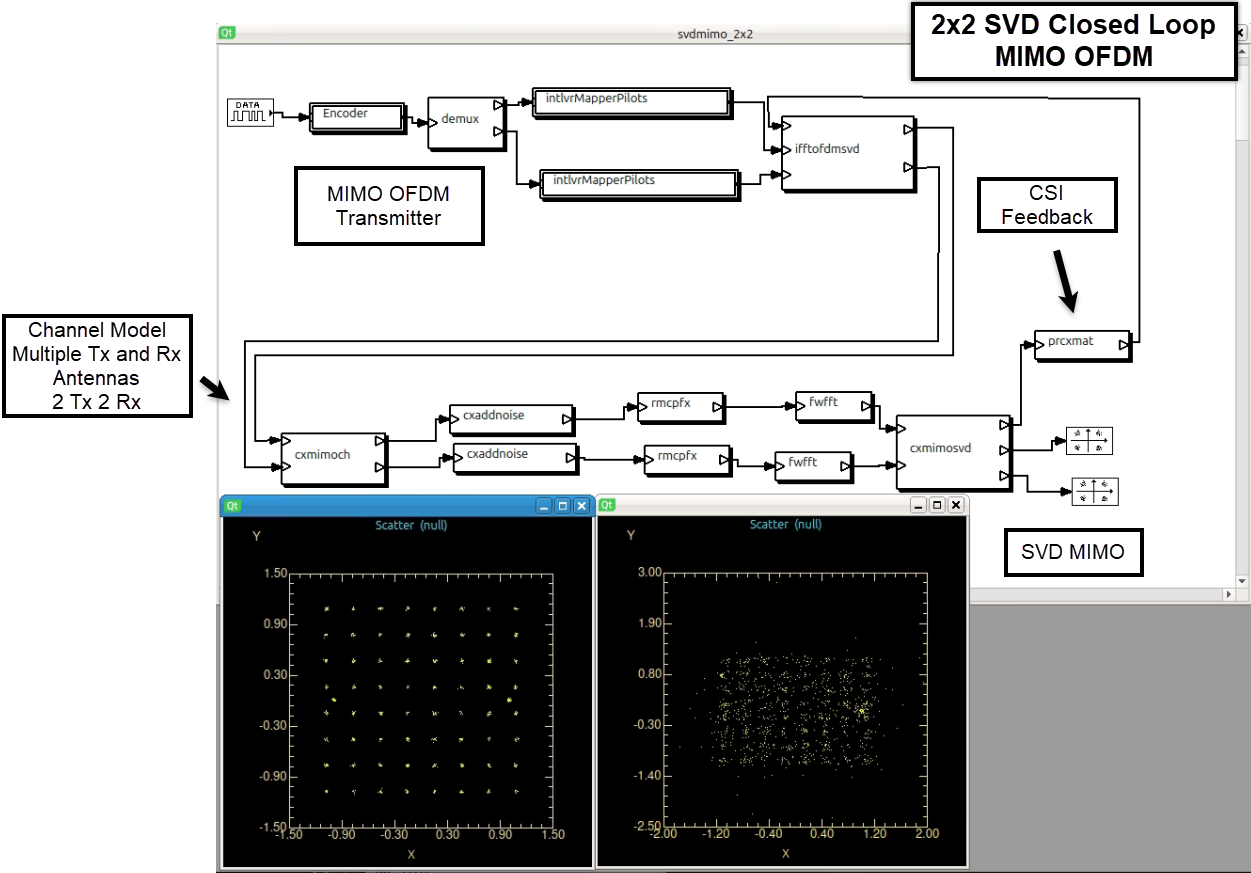
\includegraphics [width=4in]{./Figures/svd-mimo-2x2.png}
  \caption{Capsim® MIMO OFDM 2x2 Closed Loop with Channel Modeling and Noise Specification 
}
  \label{fig:mimo-ofdm-2x2}
\end{figure}


As show in Figures \ref{fig:svd-2x2-lapack-high-snr}  and \ref{fig:svd-2x2-cordic_fxp-high-snr}  the fixed point CORDIC based 2x2 SVD MIMO OFDM system performs well compared to the floating point LAPACK based 2x2 SVD. The slight apparent degradation is due to the finite precision in the fixed point CORDIC 2x2 SVD implementation.

A key comparison is the case where channel noise is added. In this case, we expect that the finite precision fixed point CORDIC SVD will enhance noise and degrade performance compared to the floating point LAPACK implementation. This is shown in Figures  \ref{fig:svd-2x2-lapack-medium-snr}  and  \ref{fig:svd-2x2-cordic_fxp-medium-snr} where noise variance of 1e-5 $(10^{-5}$)
  was added to each receive chain.
  
  
\begin{figure}[hbtp]
  \centering 
    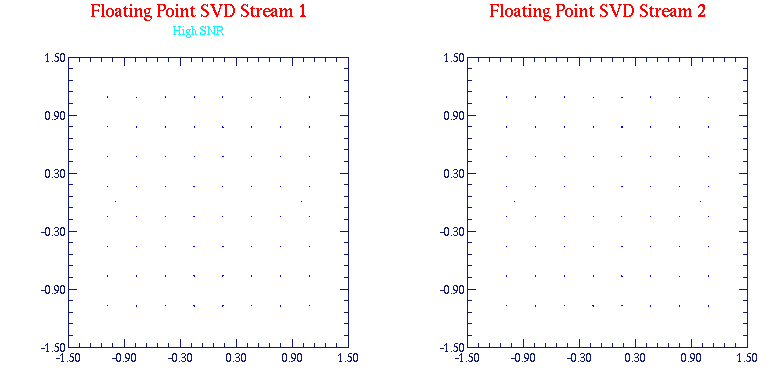
\includegraphics [width=4in]{./Figures/svd_2x2_lapack.png}
  \caption{2x2 Beam Forming MIMO OFDM 64 QAM Constellations for Each Stream LAPACK Floating Point Library, High SNR }
  \label{fig:svd-2x2-lapack-high-snr}
\end{figure}



\begin{figure}[hbtp]
  \centering 
    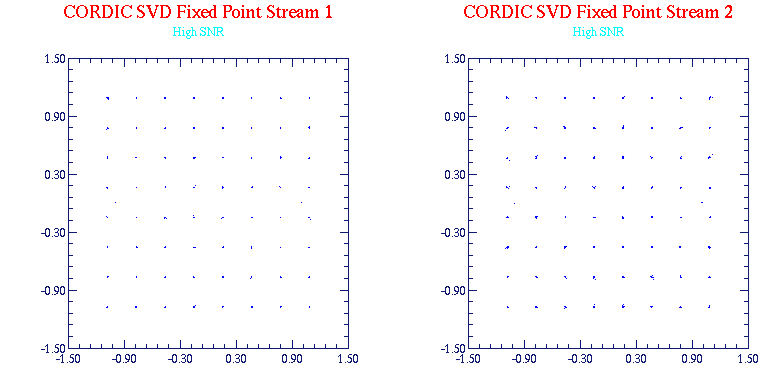
\includegraphics [width=4in]{./Figures/svd_2x2-fixed-point-cordic.png}
  \caption{2x2 Beam Forming MIMO OFDM 64 QAM Constellations for Each Stream CORDIC Fixed Point  2x2 SVD , High SNR }
  \label{fig:svd-2x2-cordic_fxp-high-snr}
\end{figure}


\begin{figure}[hbtp]
  \centering 
    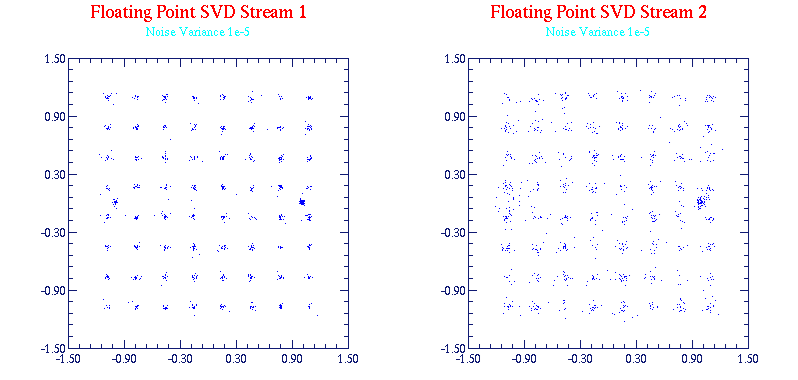
\includegraphics [width=4in]{./Figures/svd-2x2-lapack-noise-added.png}
  \caption{2x2 Beam Forming MIMO OFDM 64 QAM Constellations for Each Stream LAPACK Floating Point Library, Medium SNR }
  \label{fig:svd-2x2-lapack-medium-snr}
\end{figure}



\begin{figure}[hbtp]
  \centering 
    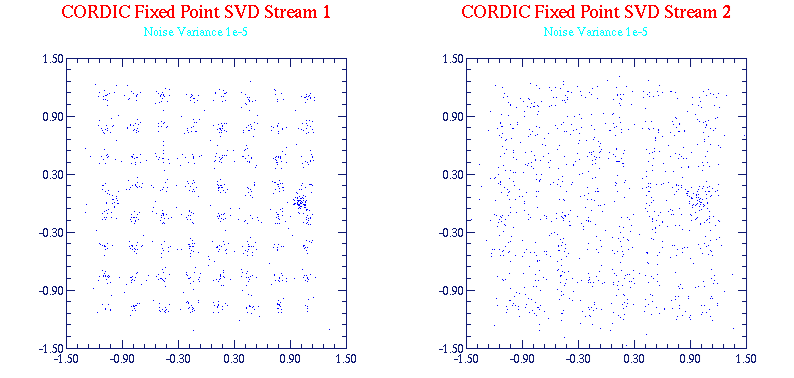
\includegraphics [width=4in]{./Figures/svd-2x2-fixed-point-cordic-noise-added.png}
  \caption{2x2 Beam Forming MIMO OFDM 64 QAM Constellations for Each Stream CORDIC Fixed Point  2x2 SVD , Medium SNR }
  \label{fig:svd-2x2-cordic_fxp-medium-snr}
\end{figure}


\section{SVD Singular Value Ratio  Comparing  Floating Point LAPACK versus Fixed Point CORDIC 2x2 SVD}

To show that the fixed point CORDIC 2x2 SVD tracks the floating point SVD in a 2x2 MIMO OFDM system we show the plot of the ratio of Singular Values for various carriers (52 for IEEE 802.11a streams) in  Figure \ref{fig:svd-radio-fxp-float}  with additive noise(variance 1e-5). Note that the ratios track very well over the 52 carriers. The deviation is at the high Singular Value Ratio which corresponds to an ill conditioned channel at that carrier frequency. The enhancement of roundoff noise is caused at this point and other ill conditioned channel conditions. 

\begin{figure}[hbtp]
  \centering 
    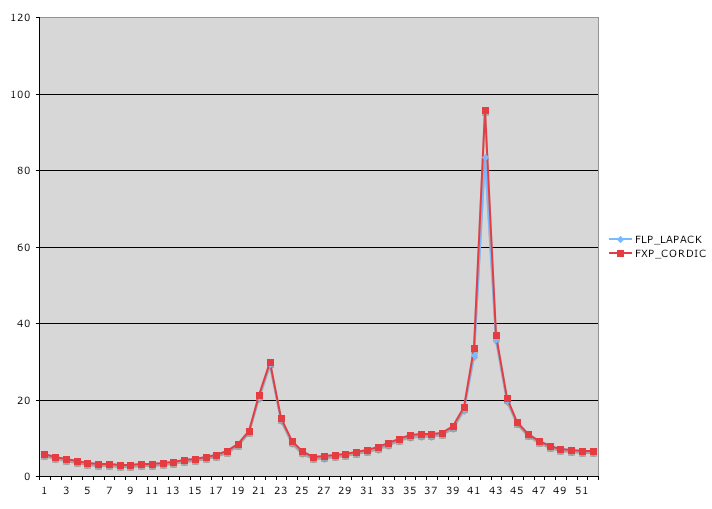
\includegraphics [width=4in]{./Figures/SVD_Ratio_Fixed-Point-Vewrsus-Floating-Point-Carriers.png}
  \caption{Singular Value Ratio: Floating Point versus Fixed Point 2x2 Closed Loop for Each Carrier(52)}
  \label{fig:svd-radio-fxp-float}
\end{figure}
\section{On the perfrormance of Open Loop MIMO  Systems}

In \cite{Gao} the Maximium to Minimum Singular Value Ratio (MMSVR) is defined. It is shown that it is a key predictor of the performance of Open-Loop MIMO OFDM systems over many channel realizations. In Figure \ref{fig:mmsvr-probability-3x3-3x4}, it is shown that for 3x4 MIMO OFDM the probability of the MMSVR is shifted to the left (lower values, less ill conditioned situations) compared to the 3x3 Open Loop system. Track the peak value to see this result. Since we can implement an Open Loop MIMO system with an SVD computation engine, and we have shown the performance of fixed point CORDIC SVD with noise and degradation due to high MMSVR, adding an extra receive antenna (3x4 versus 3x3) can greatly improve the performance of the fixed point CORDIC implementation. For example a 4x2 Closed Loop MIMO-OFDM should decrease the MMSVR and is recommended for fixed point implementation.

\begin{figure}[hbtp]
  \centering 
    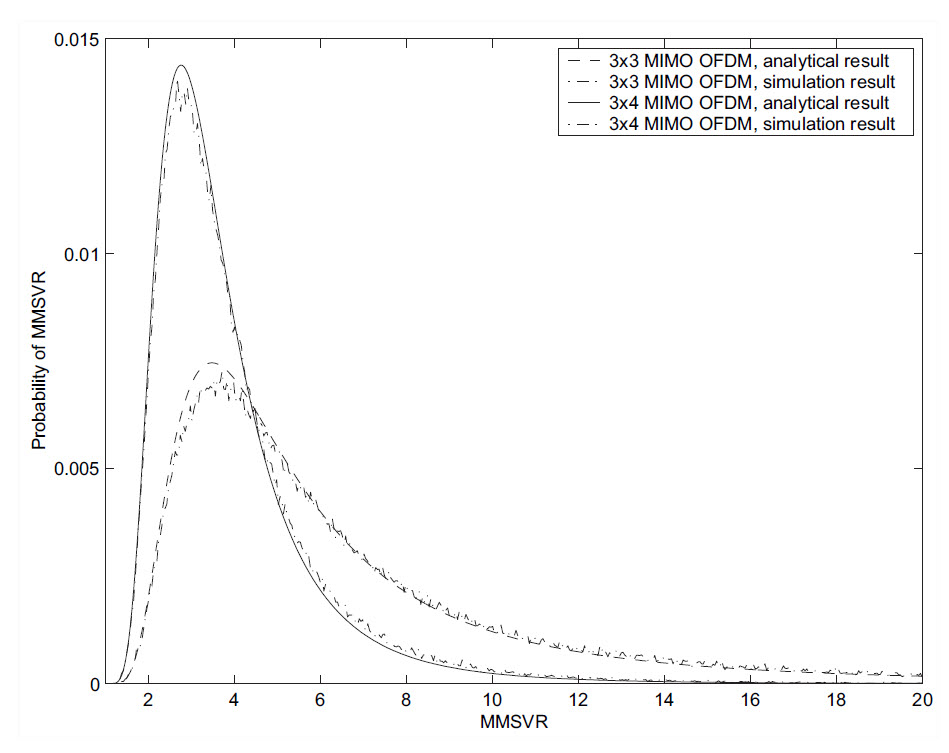
\includegraphics [width=4in]{./Figures/mmsvr-probability-3x3-3x4.jpg}
  \caption{Analytical and simulated probability density of MMSVR for 3 × 3 and 3 × 4 MIMO OFDM configurations \cite{Gao}.}
  \label{fig:mmsvr-probability-3x3-3x4}
\end{figure}

The throughput comparison of MIMO-OFDM systems at 20MHz for 3x3 and 3x4 systems is shown in Figure  \ref{fig:3x3-versus-3x4-maltsev.jpg} due to A. Maltsev and A. Davydov( see reference [19] in \cite{Gao}. Note the performance advantage of 3x4 over 3x3 MIMO OFDM as shown in the Figure are predicted analytically by the MMSVR in \cite{Gao}.


\begin{figure}[hbtp]
  \centering 
    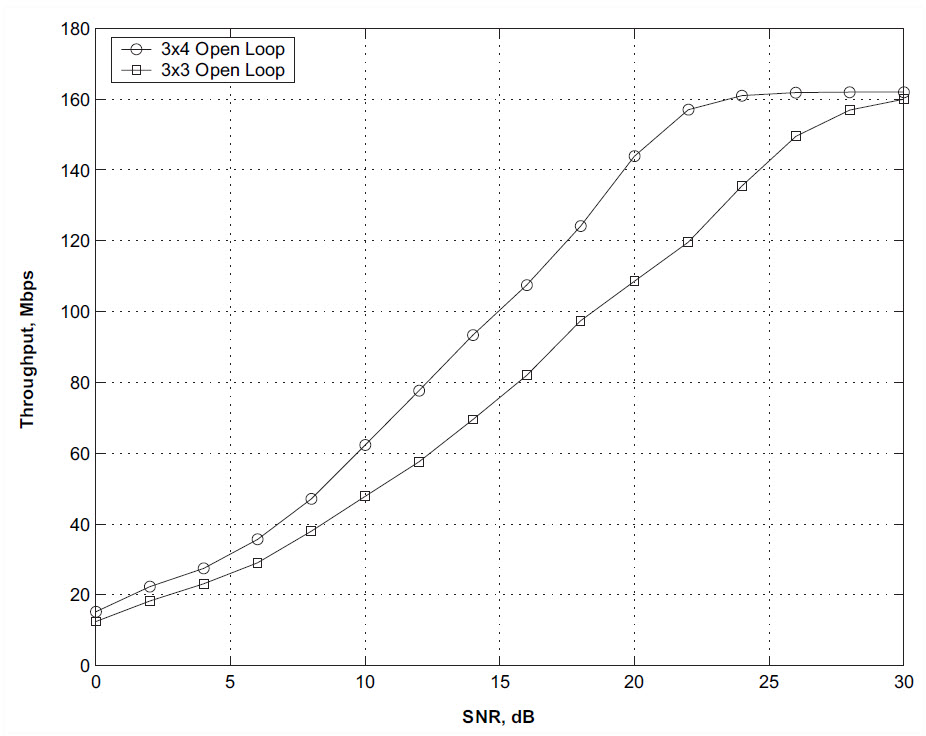
\includegraphics [width=4in]{./Figures/3x3-versus-3x4-maltsev.jpg}
  \caption{Throughput comparison of MIMO-OFDM systems at 20MHz Reference 19 in\cite{Gao}}
  \label{fig:3x3-versus-3x4-maltsev.jpg}
\end{figure}

For a demonstration of adding a receive chain to a  2x2  Open Loop MIMO-OFDM showing performance enhancement, see the video on Open Loop 2x2 and 2x3 MIMO-OFDM Systems \cite{capsim-mimo}.


\newpage




\chapter{MIMO OFDM Repository}
\paragraph{}
A full implementation of the fixed point SVD computation in  MIMO-OFDM systems is provided in the Capsim® based Block Diagram Modeling and Simulation environment at the GitHub Repository\cite{sdsp}:
\paragraph{}
        https://github.com/silicondsp/mimo-ofdm-release
\paragraph{}
The Capsim® simulation includes both Open Loop MIMO-OFDM systems and Closed Loop MIMO-OFDM systems with CSI feedback. Floating point implementations using LAPACK for matrix operations are also included for comparison with fixed point CORDIC operation implementations.












\newpage


\bibliographystyle{plain}


\bibliography{MIMO-OFDM_SVD_CORDIC_Operations}


\pagebreak
\chapter{GNU Free Documentation License}
GNU Free Documentation License
Version 1.3, 3 November 2008
\par
\noindent
Copyright \copyright  2000, 2001, 2002, 2007, 2008 Free Software Foundation, Inc.  <http://fsf.org/>
Everyone is permitted to copy and distribute verbatim copies of this license document, but changing it is not allowed.

\section{0. PREAMBLE}


The purpose of this License is to make a manual, textbook, or other functional and useful document "free" in the sense of freedom: to assure everyone the effective freedom to copy and redistribute it, with or without modifying it, either commercially or noncommercially. Secondarily, this License preserves for the author and publisher a way to get credit for their work, while not being considered responsible for modifications made by others.\\
This License is a kind of "copyleft", which means that derivative works of the document must themselves be free in the same sense. It complements the GNU General Public License, which is a copyleft license designed for free software.\\
We have designed this License in order to use it for manuals for free software, because free software needs free documentation: a free program should come with manuals providing the same freedoms that the software does. But this License is not limited to software manuals; it can be used for any textual work, regardless of subject matter or whether it is published as a printed book. We recommend this License principally for works whose purpose is instruction or reference.\\
\section{1. APPLICABILITY AND DEFINITIONS}


This License applies to any manual or other work, in any medium, that contains a notice placed by the copyright holder saying it can be distributed under the terms of this License. Such a notice grants a world-wide, royalty-free license, unlimited in duration, to use that work under the conditions stated herein. The "Document", below, refers to any such manual or work. Any member of the public is a licensee, and is addressed as "you". You accept the license if you copy, modify or distribute the work in a way requiring permission under copyright law.
A "Modified Version" of the Document means any work containing the Document or a portion of it, either copied verbatim, or with modifications and/or translated into another language.\\
A "Secondary Section" is a named appendix or a front-matter section of the Document that deals exclusively with the relationship of the publishers or authors of the Document to the Document's overall subject (or to related matters) and contains nothing that could fall directly within that overall subject. (Thus, if the Document is in part a textbook of mathematics, a Secondary Section may not explain any mathematics.) The relationship could be a matter of historical connection with the subject or with related matters, or of legal, commercial, philosophical, ethical or political position regarding them.\\
The "Invariant Sections" are certain Secondary Sections whose titles are designated, as being those of Invariant Sections, in the notice that says that the Document is released under this License. If a section does not fit the above definition of Secondary then it is not allowed to be designated as Invariant. The Document may contain zero Invariant Sections. If the Document does not identify any Invariant Sections then there are none.
The "Cover Texts" are certain short passages of text that are listed, as Front-Cover Texts or Back-Cover Texts, in the notice that says that the Document is released under this License. A Front-Cover Text may be at most 5 words, and a Back-Cover Text may be at most 25 words.\\
A "Transparent" copy of the Document means a machine-readable copy, represented in a format whose specification is available to the general public, that is suitable for revising the document straightforwardly with generic text editors or (for images composed of pixels) generic paint programs or (for drawings) some widely available drawing editor, and that is suitable for input to text formatters or for automatic translation to a variety of formats suitable for input to text formatters. A copy made in an otherwise Transparent file format whose markup, or absence of markup, has been arranged to thwart or discourage subsequent modification by readers is not Transparent. An image format is not Transparent if used for any substantial amount of text. A copy that is not "Transparent" is called "Opaque".\\
Examples of suitable formats for Transparent copies include plain ASCII without markup, Texinfo input format, LaTeX input format, SGML or XML using a publicly available DTD, and standard-conforming simple HTML, PostScript or PDF designed for human modification. Examples of transparent image formats include PNG, XCF and JPG. Opaque formats include proprietary formats that can be read and edited only by proprietary word processors, SGML or XML for which the DTD and/or processing tools are not generally available, and the machine-generated HTML, PostScript or PDF produced by some word processors for output purposes only.\\
The "Title Page" means, for a printed book, the title page itself, plus such following pages as are needed to hold, legibly, the material this License requires to appear in the title page. For works in formats which do not have any title page as such, "Title Page" means the text near the most prominent appearance of the work's title, preceding the beginning of the body of the text.\\
The "publisher" means any person or entity that distributes copies of the Document to the public.\\
A section "Entitled XYZ" means a named subunit of the Document whose title either is precisely XYZ or contains XYZ in parentheses following text that translates XYZ in another language. (Here XYZ stands for a specific section name mentioned below, such as "Acknowledgements", "Dedications", "Endorsements", or "History".) To "Preserve the Title" of such a section when you modify the Document means that it remains a section "Entitled XYZ" according to this definition.\\
The Document may include Warranty Disclaimers next to the notice which states that this License applies to the Document. These Warranty Disclaimers are considered to be included by reference in this License, but only as regards disclaiming warranties: any other implication that these Warranty Disclaimers may have is void and has no effect on the meaning of this License.

\section{2. VERBATIM COPYING}



You may copy and distribute the Document in any medium, either commercially or noncommercially, provided that this License, the copyright notices, and the license notice saying this License applies to the Document are reproduced in all copies, and that you add no other conditions whatsoever to those of this License. You may not use technical measures to obstruct or control the reading or further copying of the copies you make or distribute. However, you may accept compensation in exchange for copies. If you distribute a large enough number of copies you must also follow the conditions in section 3.\\
You may also lend copies, under the same conditions stated above, and you may publicly display copies.

\section{3. COPYING IN QUANTITY}



If you publish printed copies (or copies in media that commonly have printed covers) of the Document, numbering more than 100, and the Document's license notice requires Cover Texts, you must enclose the copies in covers that carry, clearly and legibly, all these Cover Texts: Front-Cover Texts on the front cover, and Back-Cover Texts on the back cover. Both covers must also clearly and legibly identify you as the publisher of these copies. The front cover must present the full title with all words of the title equally prominent and visible. You may add other material on the covers in addition. Copying with changes limited to the covers, as long as they preserve the title of the Document and satisfy these conditions, can be treated as verbatim copying in other respects.\\
If the required texts for either cover are too voluminous to fit legibly, you should put the first ones listed (as many as fit reasonably) on the actual cover, and continue the rest onto adjacent pages.\\
If you publish or distribute Opaque copies of the Document numbering more than 100, you must either include a machine-readable Transparent copy along with each Opaque copy, or state in or with each Opaque copy a computer-network location from which the general network-using public has access to download using public-standard network protocols a complete Transparent copy of the Document, free of added material. If you use the latter option, you must take reasonably prudent steps, when you begin distribution of Opaque copies in quantity, to ensure that this Transparent copy will remain thus accessible at the stated location until at least one year after the last time you distribute an Opaque copy (directly or through your agents or retailers) of that edition to the public.\\
It is requested, but not required, that you contact the authors of the Document well before redistributing any large number of copies, to give them a chance to provide you with an updated version of the Document.

\section{4. MODIFICATIONS}




You may copy and distribute a Modified Version of the Document under the conditions of sections 2 and 3 above, provided that you release the Modified Version under precisely this License, with the Modified Version filling the role of the Document, thus licensing distribution and modification of the Modified Version to whoever possesses a copy of it. In addition, you must do these things in the Modified Version:\\
$\bullet$	A. Use in the Title Page (and on the covers, if any) a title distinct from that of the Document, and from those of previous versions (which should, if there were any, be listed in the History section of the Document). You may use the same title as a previous version if the original publisher of that version gives permission. \\
$\bullet$	B. List on the Title Page, as authors, one or more persons or entities responsible for authorship of the modifications in the Modified Version, together with at least five of the principal authors of the Document (all of its principal authors, if it has fewer than five), unless they release you from this requirement. \\
$\bullet$	C. State on the Title page the name of the publisher of the Modified Version, as the publisher. \\
$\bullet$	D. Preserve all the copyright notices of the Document. \\
$\bullet$	E. Add an appropriate copyright notice for your modifications adjacent to the other copyright notices. \\
$\bullet$	F. Include, immediately after the copyright notices, a license notice giving the public permission to use the Modified Version under the terms of this License, in the form shown in the Addendum below. \\
$\bullet$	G. Preserve in that license notice the full lists of Invariant Sections and required Cover Texts given in the Document's license notice. \\
$\bullet$	H. Include an unaltered copy of this License. \\
$\bullet$	I. Preserve the section Entitled "History", Preserve its Title, and add to it an item stating at least the title, year, new authors, and publisher of the Modified Version as given on the Title Page. If there is no section Entitled "History" in the Document, create one stating the title, year, authors, and publisher of the Document as given on its Title Page, then add an item describing the Modified Version as stated in the previous sentence. \\
$\bullet$	J. Preserve the network location, if any, given in the Document for public access to a Transparent copy of the Document, and likewise the network locations given in the Document for previous versions it was based on. These may be placed in the "History" section. You may omit a network location for a work that was published at least four years before the Document itself, or if the original publisher of the version it refers to gives permission. \\
$\bullet$	K. For any section Entitled "Acknowledgements" or "Dedications", Preserve the Title of the section, and preserve in the section all the substance and tone of each of the contributor acknowledgements and/or dedications given therein. \\
$\bullet$	L. Preserve all the Invariant Sections of the Document, unaltered in their text and in their titles. Section numbers or the equivalent are not considered part of the section titles. \\
$\bullet$	M. Delete any section Entitled "Endorsements". Such a section may not be included in the Modified Version. \\
$\bullet$	N. Do not retitle any existing section to be Entitled "Endorsements" or to conflict in title with any Invariant Section. \\
$\bullet$	O. Preserve any Warranty Disclaimers. \\
If the Modified Version includes new front-matter sections or appendices that qualify as Secondary Sections and contain no material copied from the Document, you may at your option designate some or all of these sections as invariant. To do this, add their titles to the list of Invariant Sections in the Modified Version's license notice. These titles must be distinct from any other section titles.\\
You may add a section Entitled "Endorsements", provided it contains nothing but endorsements of your Modified Version by various parties?for example, statements of peer review or that the text has been approved by an organization as the authoritative definition of a standard.
You may add a passage of up to five words as a Front-Cover Text, and a passage of up to 25 words as a Back-Cover Text, to the end of the list of Cover Texts in the Modified Version. Only one passage of Front-Cover Text and one of Back-Cover Text may be added by (or through arrangements made by) any one entity. If the Document already includes a cover text for the same cover, previously added by you or by arrangement made by the same entity you are acting on behalf of, you may not add another; but you may replace the old one, on explicit permission from the previous publisher that added the old one.
The author(s) and publisher(s) of the Document do not by this License give permission to use their names for publicity for or to assert or imply endorsement of any Modified Version.

\section{5. COMBINING DOCUMENTS}



You may combine the Document with other documents released under this License, under the terms defined in section 4 above for modified versions, provided that you include in the combination all of the Invariant Sections of all of the original documents, unmodified, and list them all as Invariant Sections of your combined work in its license notice, and that you preserve all their Warranty Disclaimers.\\
The combined work need only contain one copy of this License, and multiple identical Invariant Sections may be replaced with a single copy. If there are multiple Invariant Sections with the same name but different contents, make the title of each such section unique by adding at the end of it, in parentheses, the name of the original author or publisher of that section if known, or else a unique number. Make the same adjustment to the section titles in the list of Invariant Sections in the license notice of the combined work.
In the combination, you must combine any sections Entitled "History" in the various original documents, forming one section Entitled "History"; likewise combine any sections Entitled "Acknowledgements", and any sections Entitled "Dedications". You must delete all sections Entitled "Endorsements".

\section{6. COLLECTIONS OF DOCUMENTS}


You may make a collection consisting of the Document and other documents released under this License, and replace the individual copies of this License in the various documents with a single copy that is included in the collection, provided that you follow the rules of this License for verbatim copying of each of the documents in all other respects.
You may extract a single document from such a collection, and distribute it individually under this License, provided you insert a copy of this License into the extracted document, and follow this License in all other respects regarding verbatim copying of that document.

\section{7. AGGREGATION WITH INDEPENDENT WORKS}


A compilation of the Document or its derivatives with other separate and independent documents or works, in or on a volume of a storage or distribution medium, is called an "aggregate" if the copyright resulting from the compilation is not used to limit the legal rights of the compilation's users beyond what the individual works permit. When the Document is included in an aggregate, this License does not apply to the other works in the aggregate which are not themselves derivative works of the Document.
If the Cover Text requirement of section 3 is applicable to these copies of the Document, then if the Document is less than one half of the entire aggregate, the Document's Cover Texts may be placed on covers that bracket the Document within the aggregate, or the electronic equivalent of covers if the Document is in electronic form. Otherwise they must appear on printed covers that bracket the whole aggregate.

\section{8. TRANSLATION}


Translation is considered a kind of modification, so you may distribute translations of the Document under the terms of section 4. Replacing Invariant Sections with translations requires special permission from their copyright holders, but you may include translations of some or all Invariant Sections in addition to the original versions of these Invariant Sections. You may include a translation of this License, and all the license notices in the Document, and any Warranty Disclaimers, provided that you also include the original English version of this License and the original versions of those notices and disclaimers. In case of a disagreement between the translation and the original version of this License or a notice or disclaimer, the original version will prevail.
If a section in the Document is Entitled "Acknowledgements", "Dedications", or "History", the requirement (section 4) to Preserve its Title (section 1) will typically require changing the actual title.

\section{9. TERMINATION}


You may not copy, modify, sublicense, or distribute the Document except as expressly provided under this License. Any attempt otherwise to copy, modify, sublicense, or distribute it is void, and will automatically terminate your rights under this License.
However, if you cease all violation of this License, then your license from a particular copyright holder is reinstated (a) provisionally, unless and until the copyright holder explicitly and finally terminates your license, and (b) permanently, if the copyright holder fails to notify you of the violation by some reasonable means prior to 60 days after the cessation.
Moreover, your license from a particular copyright holder is reinstated permanently if the copyright holder notifies you of the violation by some reasonable means, this is the first time you have received notice of violation of this License (for any work) from that copyright holder, and you cure the violation prior to 30 days after your receipt of the notice.
Termination of your rights under this section does not terminate the licenses of parties who have received copies or rights from you under this License. If your rights have been terminated and not permanently reinstated, receipt of a copy of some or all of the same material does not give you any rights to use it.

\section{10. FUTURE REVISIONS OF THIS LICENSE}


The Free Software Foundation may publish new, revised versions of the GNU Free Documentation License from time to time. Such new versions will be similar in spirit to the present version, but may differ in detail to address new problems or concerns. See http://www.gnu.org/copyleft/.
Each version of the License is given a distinguishing version number. If the Document specifies that a particular numbered version of this License "or any later version" applies to it, you have the option of following the terms and conditions either of that specified version or of any later version that has been published (not as a draft) by the Free Software Foundation. If the Document does not specify a version number of this License, you may choose any version ever published (not as a draft) by the Free Software Foundation. If the Document specifies that a proxy can decide which future versions of this License can be used, that proxy's public statement of acceptance of a version permanently authorizes you to choose that version for the Document.

\section{11. RELICENSING}


?Massive Multiauthor Collaboration Site" (or "MMC Site") means any World Wide Web server that publishes copyrightable works and also provides prominent facilities for anybody to edit those works. A public wiki that anybody can edit is an example of such a server. A "Massive Multiauthor Collaboration" (or "MMC") contained in the site means any set of copyrightable works thus published on the MMC site.
"CC-BY-SA" means the Creative Commons Attribution-Share Alike 3.0 license published by Creative Commons Corporation, a not-for-profit corporation with a principal place of business in San Francisco, California, as well as future copyleft versions of that license published by that same organization.
"Incorporate" means to publish or republish a Document, in whole or in part, as part of another Document.
An MMC is "eligible for relicensing" if it is licensed under this License, and if all works that were first published under this License somewhere other than this MMC, and subsequently incorporated in whole or in part into the MMC, (1) had no cover texts or invariant sections, and (2) were thus incorporated prior to November 1, 2008.
The operator of an MMC Site may republish an MMC contained in the site under CC-BY-SA on the same site at any time before August 1, 2009, provided the MMC is eligible for relicensing.



\end{document}
